
\documentclass{standalone}
\usepackage[svgnames]{xcolor}
\usepackage{pgfplots}
\pgfplotsset{compat=newest}
\usepackage[sfdefault]{FiraSans}
\usepackage{FiraMono}
\renewcommand*\familydefault{\sfdefault}
\begin{document}
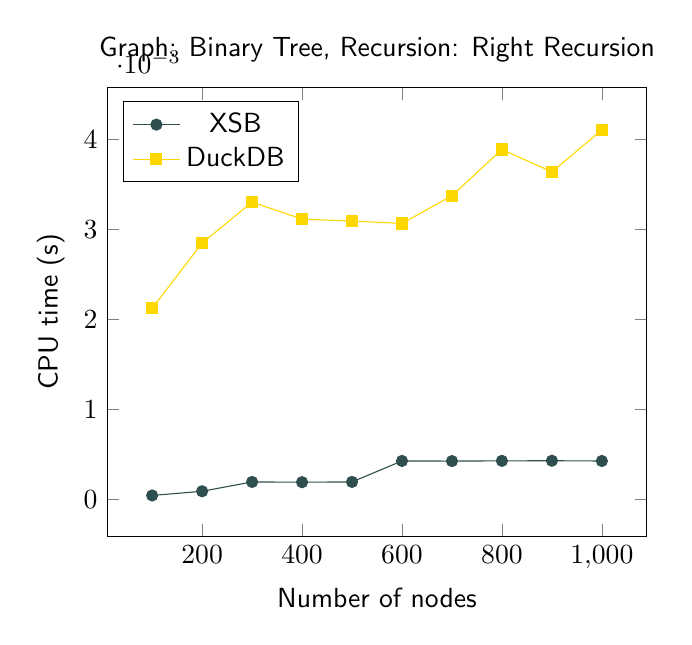
\begin{tikzpicture}
    \begin{axis}[
        title={Graph: Binary Tree, Recursion: Right Recursion},
        xlabel={Number of nodes},
        ylabel={CPU time (s)},
        legend pos={north west},
        ymax=0.004573799999999994
    ]
    \addplot+[DarkSlateGray, mark options={color=DarkSlateGray}] coordinates {(100,4.5400000000000304e-05) (200,9.180000000000021e-05) (300,0.00019540000000000022) (400,0.00019279999999999997) (500,0.00019559999999999941) (600,0.0004288) (700,0.00042719999999999965) (800,0.00042960000000000003) (900,0.0004309999999999998) (1000,0.0004281999999999998)};
\addlegendentry{XSB}
\addplot+[Gold, mark options={color=Gold}] coordinates {(100,0.002124400000000004) (200,0.0028497999999999913) (300,0.003304399999999985) (400,0.0031154000000000017) (500,0.0030948000000000087) (600,0.003067399999999998) (700,0.0033752000000000005) (800,0.0038900000000000046) (900,0.003639999999999988) (1000,0.00410640000000001)};
\addlegendentry{DuckDB}

    \end{axis}
\end{tikzpicture}
\end{document}
